% =============================================================================
% CO2-Based Occupancy Duration Inference in University Dormitory Rooms
% Target journal: Building and Environment
% =============================================================================
\documentclass[preprint,number]{elsarticle}

\usepackage[utf8]{inputenc}
\usepackage[T1]{fontenc}
\usepackage{amsmath,amssymb,amsfonts}
\usepackage{graphicx}
\usepackage{booktabs}
\usepackage{multirow}
\usepackage{siunitx}
\usepackage{xcolor}
\usepackage{lineno}
\usepackage{hyperref}
\usepackage{algorithm}
\usepackage{algpseudocode}
\usepackage{subcaption}
\usepackage{tikz}
\usetikzlibrary{arrows.meta, positioning, shapes.geometric, fit, calc, backgrounds}

% Line numbers for review (uncomment for submission)
% \modulolinenumbers[5]
% \linenumbers

% SI units setup
\sisetup{
  separate-uncertainty=true,
  multi-part-units=single,
}

\journal{Building and Environment}

\begin{document}

\begin{frontmatter}

\title{Inferring Occupancy Duration from Indoor CO\textsubscript{2} Concentrations in University Dormitory Rooms: A Block-Level Excess Approach with Monte Carlo Uncertainty Quantification}

\author[cript]{Gautam~Author\corref{cor1}}
\ead{gautam@university.edu}
\cortext[cor1]{Corresponding author}

\affiliation[cript]{organization={Center for Research in Indoor and Personal Technologies (CRIPT)},
             addressline={},
             city={},
             state={},
             postcode={},
             country={USA}}

\begin{abstract}
Estimating how long occupants spend in their rooms is valuable for understanding indoor environmental exposure, energy use, and well-being in residential buildings. While CO\textsubscript{2} concentration is widely used as a proxy for occupancy detection (present/absent), estimating \emph{duration} of occupancy within time blocks remains an open challenge. We present a physics-based method that infers occupied minutes within four-hour blocks from indoor CO\textsubscript{2} measurements in university dormitory rooms. The method fits an autoregressive AR(1) model to each sensor's CO\textsubscript{2} time series, calibrates block-level excess CO\textsubscript{2} against per-sensor empty-room behavior, and converts the calibrated signal to occupied minutes using finite-window mass balance physics. Monte Carlo propagation of parameter uncertainty yields 80\% credible intervals for each estimate. We validate the method on 12~sensors monitoring 24~subjects across 774~four-hour blocks over 68~days. All four independent evaluation criteria---covering cross-sensor generalizability (E1--E2), parameter sensitivity (E3), and uncertainty informativeness (E4)---are satisfied. Two calibration diagnostics used to tune the empty-room floor are met by construction. An out-of-sample temporal split shows that the calibration partially generalizes but degrades when training data are limited. A semisynthetic validation---injecting known occupancy patterns into real empty-room CO\textsubscript{2} data with model-mismatch stress tests---provides partial external validation of duration recovery accuracy. Comparison against threshold and slope baseline methods demonstrates that the block-excess approach achieves superior empty-room specificity. The method requires no labeled minute-level training data, uses only CO\textsubscript{2} measurements and known-empty calibration periods, and runs in under one minute on standard hardware.
\end{abstract}

\begin{keyword}
occupancy duration \sep CO\textsubscript{2} inference \sep indoor air quality \sep autoregressive model \sep Monte Carlo uncertainty \sep dormitory buildings
\end{keyword}

\end{frontmatter}

% =============================================================================
\section{Introduction}
\label{sec:introduction}
% =============================================================================

Understanding how long building occupants spend in particular spaces is fundamental to indoor environmental quality (IEQ) assessment, energy management, and occupant well-being research \cite{frontczak2012literature}. In residential buildings---particularly university dormitories where students live, study, and sleep---the duration of room occupancy directly determines cumulative exposure to indoor pollutants, thermal conditions, and lighting environments \cite{daisey2003indoor, fisk2017association}. Occupancy-driven energy models further rely on accurate time-use data to predict heating, cooling, and ventilation loads \cite{yan2015occupant, dong2018modeling}.

While numerous methods exist for binary occupancy detection (present vs.\ absent), far fewer address the more informative question of \emph{how long} an occupant was present during a given time window. Binary detection from CO\textsubscript{2} thresholds is well established \cite{candanedo2016accurate, jin2018virtual, chen2018building}, and multi-sensor fusion approaches combining CO\textsubscript{2} with temperature, humidity, and light have pushed detection accuracy above 95\% \cite{yang2014systematic}. Machine learning approaches---including random forests, support vector machines, and deep recurrent networks---have improved detection accuracy further \cite{masood2019occupancy, chen2020environmental, tekler2020occupancy} but typically still target binary or count outcomes rather than continuous duration. Bayesian and state-space formulations have been applied to CO\textsubscript{2}-based occupancy counting \cite{ebadat2015estimation, wang2018inferring}, yet these also estimate the number of people present rather than how long they stay.

CO\textsubscript{2} concentration is a particularly attractive proxy for occupancy in dormitory settings because it is noninvasive, inexpensive to measure continuously, and directly linked to human metabolic activity through respiration. The physics of indoor CO\textsubscript{2} are well understood: occupants generate CO\textsubscript{2} at rates proportional to their metabolic activity (\SIrange{12}{20}{L/h} per person at rest \cite{persily2017carbon}), while ventilation removes CO\textsubscript{2} at a rate proportional to the concentration difference between indoor and outdoor air \cite{ashrae2022standard}. This mass-balance relationship creates a direct, physics-based link between CO\textsubscript{2} dynamics and occupancy patterns and underpins demand-controlled ventilation strategies \cite{lu2010design}.

However, extracting \emph{duration} information from CO\textsubscript{2} time series faces several challenges. First, the decay time constant of indoor CO\textsubscript{2} (typically 30--120 minutes in naturally ventilated rooms) means that CO\textsubscript{2} remains elevated long after occupants depart, creating ambiguity between current and residual occupancy signal. Second, sensor noise, outdoor CO\textsubscript{2} fluctuations, and building-level ventilation transients introduce confounding variation. Third, the generation rate per occupant depends on metabolic activity, which varies with activity type and individual physiology.

In this paper, we present a method that addresses these challenges by operating at the \emph{block level} (four-hour windows) rather than attempting minute-by-minute occupancy reconstruction. This design choice is motivated by a fundamental signal-to-noise ratio (SNR) argument: at the minute timescale, the occupancy-driven CO\textsubscript{2} innovation (typically \SIrange{5}{60}{ppm/min}) is comparable to or smaller than sensor noise (\SIrange{5}{40}{ppm}), yielding minute-level SNR of order unity. At the block level, averaging over 240 minutes reduces \emph{innovation} noise, though the AR(1) autocorrelation ($\hat{\phi} \approx 0.995$) limits the effective noise reduction compared to the i.i.d.\ case; the practical gain comes from aggregating the cumulative CO\textsubscript{2} signal over a long window rather than from simple $\sqrt{n}$ averaging.

The contributions of this paper are:
\begin{enumerate}
    \item A physics-based method for estimating occupancy \emph{duration} (not just presence/absence) from CO\textsubscript{2}, requiring no labeled minute-level training data---only binary block-level presence labels and known-empty calibration periods.
    \item Per-sensor adaptive calibration that accounts for room-specific ventilation, sensor placement, and residual CO\textsubscript{2} characteristics.
    \item Full Monte Carlo uncertainty quantification providing 80\% credible intervals for each block-level duration estimate.
    \item A structured validation framework distinguishing calibration diagnostics from independent evaluation criteria for CO\textsubscript{2}-based duration estimation.
    \item Application to 24 university dormitory residents across 12 rooms over 68 days, demonstrating feasibility in real-world conditions.
\end{enumerate}

Fig.~\ref{fig:method_overview} provides an overview of the proposed method.

\begin{figure}[htbp]
    \centering
    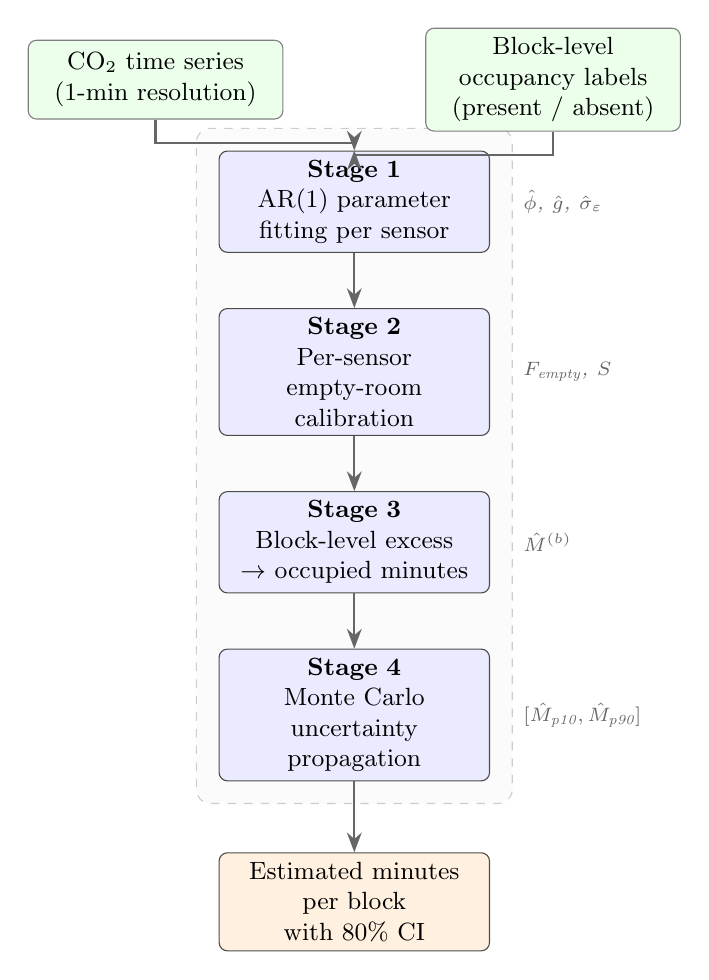
\begin{tikzpicture}[
        node distance=0.6cm and 1.2cm,
        block/.style={rectangle, draw=black!70, fill=blue!8, text width=3.2cm, minimum height=1.1cm, align=center, rounded corners=3pt, font=\small},
        data/.style={rectangle, draw=black!50, fill=green!8, text width=3.0cm, minimum height=1.0cm, align=center, rounded corners=3pt, font=\small},
        output/.style={rectangle, draw=black!70, fill=orange!12, text width=3.2cm, minimum height=1.1cm, align=center, rounded corners=3pt, font=\small},
        arrow/.style={-{Stealth[length=2.5mm]}, thick, draw=black!60},
        label/.style={font=\scriptsize\itshape, text=black!60},
    ]
        % Data inputs
        \node[data] (co2) {CO\textsubscript{2} time series\\(1-min resolution)};
        \node[data, right=1.8cm of co2] (labels) {Block-level\\occupancy labels\\(present / absent)};

        % Processing steps
        \node[block, below=0.9cm of $(co2)!0.5!(labels)$] (fit) {\textbf{Stage 1}\\AR(1) parameter\\fitting per sensor};
        \node[block, below=0.7cm of fit] (calibrate) {\textbf{Stage 2}\\Per-sensor\\empty-room\\calibration};
        \node[block, below=0.7cm of calibrate] (estimate) {\textbf{Stage 3}\\Block-level excess\\$\to$ occupied minutes};
        \node[block, below=0.7cm of estimate] (mc) {\textbf{Stage 4}\\Monte Carlo\\uncertainty\\propagation};

        % Outputs
        \node[output, below=0.9cm of mc] (result) {Estimated minutes\\per block\\with 80\% CI};

        % Parameter labels on the right
        \node[label, right=0.3cm of fit] {$\hat{\phi}$, $\hat{g}$, $\hat{\sigma}_\varepsilon$};
        \node[label, right=0.3cm of calibrate] {$F_\text{empty}$, $S$};
        \node[label, right=0.3cm of estimate] {$\hat{M}^{(b)}$};
        \node[label, right=0.3cm of mc] {$[\hat{M}_\text{p10}, \hat{M}_\text{p90}]$};

        % Arrows
        \draw[arrow] (co2.south) -- ++(0,-0.3) -| (fit.north);
        \draw[arrow] (labels.south) -- ++(0,-0.3) -| (fit.north);
        \draw[arrow] (fit) -- (calibrate);
        \draw[arrow] (calibrate) -- (estimate);
        \draw[arrow] (estimate) -- (mc);
        \draw[arrow] (mc) -- (result);

        % Background grouping
        \begin{scope}[on background layer]
            \node[fit=(fit)(calibrate)(estimate)(mc), draw=black!20, dashed, rounded corners=5pt, inner sep=8pt, fill=gray!3] {};
        \end{scope}
    \end{tikzpicture}
    \caption{Overview of the proposed method. CO\textsubscript{2} time series and block-level occupancy labels are processed through four stages: (1) per-sensor AR(1) parameter fitting, (2) empty-room calibration, (3) block-level excess-to-duration conversion, and (4) Monte Carlo uncertainty quantification. The output is an estimated number of occupied minutes per four-hour block with an 80\% credible interval.}
    \label{fig:method_overview}
\end{figure}

% =============================================================================
\section{Methods}
\label{sec:methods}
% =============================================================================

% -----------------------------------------------------------------------------
\subsection{Study design and data collection}
\label{sec:study_design}
% -----------------------------------------------------------------------------

Data were collected from a university dormitory building as part of the Center for Research in Indoor and Personal Technologies (CRIPT) study. The study monitored indoor CO\textsubscript{2} concentrations and occupancy patterns in student rooms over a 68-day period from February~4 to April~13, 2025.

\subsubsection{CO\textsubscript{2} monitoring}

Indoor CO\textsubscript{2} concentrations were measured at one-minute intervals using nondispersive infrared (NDIR) sensors deployed in each monitored room. A total of 78~sensors recorded approximately 1.4~million minute-level observations across 138~data files. Of these, 12~sensors were matched to rooms with concurrent occupancy ground truth, providing the dataset for method development and validation.

The 12~sensors monitored rooms of two types: 9~single-occupancy rooms and 3~shared rooms (two assigned residents). Sensors were placed at desk height to capture the breathing zone CO\textsubscript{2} concentration representative of the occupied microenvironment.

\subsubsection{Occupancy ground truth}

Self-reported occupancy data were collected from 24~participants (two per single room, two per shared room) through a structured survey instrument. Each single-occupancy room has one assigned resident; however, two study participants were enrolled per room to provide independent survey responses. The CO\textsubscript{2} sensor measures the room environment and cannot distinguish individual occupants, so the CO\textsubscript{2}-based duration estimate for a given block is the same for all participants associated with a sensor. Participant-level totals differ only because they are aggregated over different subsets of blocks based on each participant's self-reported presence schedule. Participants reported their presence or absence for each four-hour block of the day (02:00--06:00, 06:00--10:00, 10:00--14:00, 14:00--18:00, 18:00--22:00, 22:00--02:00), yielding a binary label for each block: 1 (present for some or all of the block) or 0 (absent for the entire block).

The ground truth thus provides block-level \emph{presence} labels but not the exact number of minutes present within each block. This distinction is important: a label of 1 indicates that the subject was present for at least some portion of the four-hour block, which could range from a few minutes to the full 240 minutes.

\subsubsection{Dataset summary}

After matching CO\textsubscript{2} sensors to subjects with occupancy labels, the analysis dataset comprises 791~four-hour blocks: 539~blocks labeled as present (label = 1) and 252~blocks labeled as absent (label = 0). Of these, 774~blocks (535~present, 239~absent) had overlapping CO\textsubscript{2} data and produced duration estimates; the remaining 17~blocks were excluded because the sensor data did not cover the block's time window. Table~\ref{tab:data_summary} summarizes the dataset characteristics.

\begin{table}[htbp]
\centering
\caption{Dataset summary statistics.}
\label{tab:data_summary}
\begin{tabular}{lr}
\toprule
Characteristic & Value \\
\midrule
Monitoring period & Feb 4 -- Apr 13, 2025 \\
Duration (days) & 68 \\
Number of sensors & 12 \\
\quad Single-occupancy rooms & 9 \\
\quad Shared rooms & 3 \\
Number of subjects & 24 \\
Total four-hour blocks & 791 \\
\quad Present (label = 1) & 539 \\
\quad Absent (label = 0) & 252 \\
CO\textsubscript{2} minute-level observations & ${\sim}1.4 \times 10^6$ \\
\bottomrule
\end{tabular}
\end{table}

% -----------------------------------------------------------------------------
\subsection{CO\textsubscript{2} dynamics model}
\label{sec:co2_model}
% -----------------------------------------------------------------------------

We model indoor CO\textsubscript{2} concentration using a discrete-time autoregressive AR(1) process that captures the essential physics of indoor CO\textsubscript{2} generation and removal. Let $C_t$ denote the smoothed CO\textsubscript{2} concentration at minute $t$ and $C_b$ denote the ambient baseline concentration. The excess CO\textsubscript{2} above baseline is defined as:
\begin{equation}
    E_t = \max(C_t - C_b, \; 0)
    \label{eq:excess}
\end{equation}

The AR(1) dynamics relate consecutive excess values:
\begin{equation}
    E_t = \phi \, E_{t-1} + g \cdot O_t + \varepsilon_t
    \label{eq:ar1}
\end{equation}
where $\phi \in (0, 1)$ is the decay parameter (related to the air exchange rate), $g > 0$ is the CO\textsubscript{2} generation rate per minute of occupancy (ppm/min), $O_t \in \{0, 1\}$ is the occupancy state at minute $t$, and $\varepsilon_t \sim \mathcal{N}(0, \sigma_\varepsilon^2)$ is the innovation noise.

\subsubsection{Physical interpretation of model parameters}

The decay parameter $\phi$ captures the fraction of excess CO\textsubscript{2} that persists from one minute to the next. It is related to the effective air exchange rate $\lambda$ (in air changes per minute) by $\phi = 1 - \lambda$. For typical dormitory rooms with natural or mechanical ventilation, $\lambda$ ranges from 0.005 to 0.03 per minute (\SIrange{0.3}{1.8}{ACH}), corresponding to $\phi \in [0.97, 0.995]$.

The generation rate $g$ represents the CO\textsubscript{2} emission rate of the room's occupant(s) expressed as the concentration increase per minute of presence. At steady state with continuous single-person occupancy, the excess CO\textsubscript{2} converges to:
\begin{equation}
    E_\text{ss} = \frac{g}{1 - \phi}
    \label{eq:steady_state}
\end{equation}

For example, with $g = \SI{15}{ppm/min}$ and $\phi = 0.995$, the steady-state excess would be $15/0.005 = \SI{3000}{ppm}$ above baseline---though in practice, occupancy is intermittent and steady state is rarely achieved.

The innovation noise $\sigma_\varepsilon$ captures sensor measurement error, short-term CO\textsubscript{2} fluctuations from sources other than occupancy (cooking, open windows, corridor air mixing), and model misspecification.

\subsubsection{Baseline estimation}

The ambient baseline $C_b$ is estimated as the 1st percentile of all CO\textsubscript{2} readings for each sensor across its entire monitoring period. This captures the true outdoor/ambient air level (${\sim}\SIrange{400}{420}{ppm}$) rather than the potentially elevated concentrations during nominally ``empty'' periods when residual CO\textsubscript{2} from prior occupancy may still be present. A floor of \SI{380}{ppm} is enforced to ensure physical plausibility.

% -----------------------------------------------------------------------------
\subsection{Parameter estimation}
\label{sec:param_estimation}
% -----------------------------------------------------------------------------

For each sensor, we estimate $\phi$, $g$, and $\sigma_\varepsilon$ from the minute-level CO\textsubscript{2} time series using the known-empty (label = 0) and known-occupied (label = 1) periods.

\subsubsection{Room-level occupancy labels for shared rooms}

For single-occupancy rooms, the subject-level occupancy label directly indicates whether the room is empty.  For shared rooms (two subjects per sensor), the subject-level label reflects individual presence, not room-level emptiness: a minute where subject~A is absent but subject~B is present still has elevated CO\textsubscript{2}.  We therefore compute a room-level occupancy indicator for each sensor--minute pair:
\begin{equation}
    O_t^\text{room} = \max_{j \in \mathcal{J}_s} O_{j,t}
    \label{eq:room_present}
\end{equation}
where $\mathcal{J}_s$ is the set of subjects mapped to sensor~$s$.  All physics fitting (decay rate, noise, empty-room floor) uses $O_t^\text{room} = 0$ to identify truly-empty minutes, preventing label contamination in shared rooms.

\subsubsection{Decay parameter ($\phi$)}

The decay parameter is estimated from CO\textsubscript{2} decay episodes during known-empty periods. We select consecutive minute pairs where (i) the room is labeled absent, (ii) the time gap is exactly one minute (no data gaps), and (iii) the preceding excess exceeds \SI{30}{ppm} (ensuring we fit genuine CO\textsubscript{2} decay rather than noise near ambient). The ordinary least squares (OLS) estimator is:
\begin{equation}
    \hat{\phi}_\text{OLS} = \frac{\sum_{t \in \mathcal{D}} E_{t-1} \, E_t}{\sum_{t \in \mathcal{D}} E_{t-1}^2}
    \label{eq:phi_ols}
\end{equation}
where $\mathcal{D}$ denotes the set of valid decay observations. The standard error is:
\begin{equation}
    \text{SE}(\hat{\phi}) = \sqrt{\frac{\hat{\sigma}_\varepsilon^2}{\sum_{t \in \mathcal{D}} E_{t-1}^2}}, \quad \hat{\sigma}_\varepsilon^2 = \frac{1}{|\mathcal{D}| - 1} \sum_{t \in \mathcal{D}} (E_t - \hat{\phi}_\text{OLS} \, E_{t-1})^2
    \label{eq:phi_se}
\end{equation}

With one-minute sampling, OLS estimates of $\phi$ are biased upward toward 1.0 due to extreme autocorrelation. We apply Bayesian shrinkage toward a physical prior ($\phi_\text{prior} = 0.97$, corresponding to ${\sim}0.03$ air changes per minute):
\begin{equation}
    \hat{\phi} = \lambda_s \, \phi_\text{prior} + (1 - \lambda_s) \, \hat{\phi}_\text{OLS}, \quad \lambda_s = \frac{w_\text{prior}}{w_\text{prior} + |\mathcal{D}|}
    \label{eq:phi_shrinkage}
\end{equation}
where $w_\text{prior} = 180$ is the effective prior sample size. The final estimate is clipped to $[\phi_\text{min}, \phi_\text{max}] = [0.85, 0.995]$.

\subsubsection{Generation rate ($g$)}

The generation rate is estimated using the steady-state relationship between excess CO\textsubscript{2} and occupancy. During occupied periods, the 75th percentile of excess CO\textsubscript{2} serves as a proxy for sustained-presence conditions:
\begin{equation}
    \hat{g} = \max\!\left(\left(E_\text{occ}^{(75)} - \tilde{E}_\text{empty}\right) \cdot (1 - \hat{\phi}), \;\; \hat{g}_\text{innov}, \;\; \SI{1.0}{ppm/min}\right)
    \label{eq:g_hat}
\end{equation}
where $E_\text{occ}^{(75)}$ is the 75th percentile of excess during occupied minutes, $\tilde{E}_\text{empty}$ is the median excess during empty minutes, and $\hat{g}_\text{innov}$ is an alternative estimate from the quantile of positive innovations during occupied periods. The generation rate is clipped to $[\SI{1.0}{}, \SI{60.0}{ppm/min}]$.

\subsubsection{Innovation noise ($\sigma_\varepsilon$)}

The innovation noise is estimated as the standard deviation of innovations during known-empty, consecutive-minute periods:
\begin{equation}
    \hat{\sigma}_\varepsilon = \text{SD}\!\left(\{E_t - \hat{\phi} \, E_{t-1} : t \in \mathcal{E}, \; \Delta t = 1\}\right)
    \label{eq:sigma_noise}
\end{equation}
where $\mathcal{E}$ is the set of known-empty observations. This is clipped to $[\SI{5}{}, \SI{200}{ppm}]$.

\subsubsection{Fallback parameter rules}

When a sensor has insufficient data for reliable parameter estimation, fallback values are used:
\begin{itemize}
    \item If $|\mathcal{D}| < 30$ (fewer than 30 valid decay observations): $\hat{\phi} = \phi_\text{prior} = 0.97$, $\text{SE}(\hat{\phi}) = 0.03$.
    \item If $|\mathcal{O}| < 20$ (fewer than 20 occupied-period observations): $\hat{g}$ defaults to the room-type mean (\SI{10}{ppm/min} for single rooms, \SI{18}{ppm/min} for shared rooms), $\text{SE}(\hat{g}) = 4.0$.
\end{itemize}
Sensor 20233681 uses the fallback for $\hat{\phi}$ ($n_\text{decay} = 0$) and its generation rate $\hat{g} = \SI{60}{ppm/min}$ reflects the upper clipping bound rather than sensor-specific fitting.  Table~\ref{tab:sensor_params} identifies which sensors use fallback parameters.

% -----------------------------------------------------------------------------
\subsection{Block-level excess estimation}
\label{sec:block_estimation}
% -----------------------------------------------------------------------------

The core estimation method operates at the four-hour block level, converting mean excess CO\textsubscript{2} within each block to estimated occupied minutes. The method consists of three stages: per-sensor empty-room calibration, self-normalizing scale computation, and occupied minutes estimation.

\subsubsection{Per-sensor empty-room calibration}

For each sensor, we compute block-level mean excess CO\textsubscript{2} for all blocks and establish an ``empty-room floor'' from the known-empty (label = 0) blocks. The empty-room floor captures residual CO\textsubscript{2} from prior occupancy, sensor offset, and building HVAC effects:
\begin{equation}
    F_\text{empty} = \bar{E}_{\text{empty}} + k \cdot s_{\text{empty}}
    \label{eq:empty_floor}
\end{equation}
where $\bar{E}_\text{empty}$ and $s_\text{empty}$ are the mean and standard deviation of block-mean excess across known-empty blocks, and $k$ is a floor multiplier that controls the boundary between residual CO\textsubscript{2} and genuine occupancy signal.

\paragraph{Selection of floor multiplier ($k$).}
The floor multiplier determines how aggressively residual CO\textsubscript{2} is suppressed. Because the finite-window normalization (Eq.~\ref{eq:finite_window}) maps a given excess to more inferred minutes than steady-state normalization would, the empty-room floor must be raised correspondingly to maintain empty-room specificity. We selected $k$ by a pre-specified grid search over $k \in [0.67, 1.00]$ in increments of 0.02, evaluating the calibration diagnostics C1 ($< \SI{15}{min}$) and C2 ($> 60\%$). We chose the \emph{smallest} $k$ satisfying both criteria while preserving non-degenerate sensitivity, operationalized as a substantial fraction of label = 1 blocks retaining a positive estimated duration. This procedure selected $k = 0.86$; at this value, 47\% of occupied blocks produce nonzero duration estimates.

\subsubsection{Self-normalizing scale}

Converting excess CO\textsubscript{2} to occupied fraction requires a normalization scale representing the expected block-mean excess during full continuous occupancy. Because occupancy blocks are finite (240 minutes) and steady state is rarely reached at high $\hat{\phi}$, we use a finite-window expected mean excess rather than the steady-state value $g/(1-\phi)$. For an AR(1) process with continuous occupancy over $n$ minutes, the expected block-mean excess is:
\begin{equation}
    \bar{E}_\text{full}(n) = \frac{\hat{g}}{1 - \hat{\phi}} \left[ 1 - \frac{\hat{\phi}\,(1 - \hat{\phi}^{\,n})}{n\,(1 - \hat{\phi})} \right]
    \label{eq:finite_window}
\end{equation}
We then blend this physics-based scale with a data-driven component:
\begin{equation}
    S = \frac{1}{2} \left( E_\text{occ}^{(75)} - F_\text{empty} \right) + \frac{1}{2} \cdot \bar{E}_\text{full}(n)
    \label{eq:scale}
\end{equation}
where $E_\text{occ}^{(75)}$ is the 75th percentile of block-mean excess during known-occupied blocks and $n = 240$ is the block duration in minutes. The finite-window correction is substantial at high $\hat{\phi}$: for $\hat{\phi} = 0.995$ and $n = 240$, $\bar{E}_\text{full}$ is approximately 42\% of the steady-state value $g/(1-\phi)$. The data-driven component makes cross-sensor estimates comparable even when $\hat{g}$ and $\hat{\phi}$ differ substantially between sensors, while the physics component prevents degenerate cases.

\subsubsection{Occupied minutes estimation}

For each four-hour block, the calibrated excess is computed and converted to estimated occupied minutes:
\begin{align}
    E_\text{cal}^{(b)} &= \max\!\left(\bar{E}^{(b)} - F_\text{empty}, \; 0\right) \label{eq:cal_excess} \\
    f^{(b)} &= \min\!\left(\frac{E_\text{cal}^{(b)}}{S}, \; 1\right) \label{eq:occ_fraction} \\
    \hat{M}^{(b)} &= f^{(b)} \times 240 \label{eq:minutes}
\end{align}
where $\bar{E}^{(b)}$ is the mean excess for block $b$, $E_\text{cal}^{(b)}$ is the calibrated excess after subtracting the empty-room floor, $f^{(b)}$ is the estimated occupied fraction (clipped to $[0, 1]$), and $\hat{M}^{(b)}$ is the estimated occupied minutes (out of 240 minutes per block). The complete estimation pipeline is illustrated in Fig.~\ref{fig:estimation_pipeline}, and Fig.~\ref{fig:physics_illustration} shows the model physics on example data.

\begin{figure}[htbp]
    \centering
    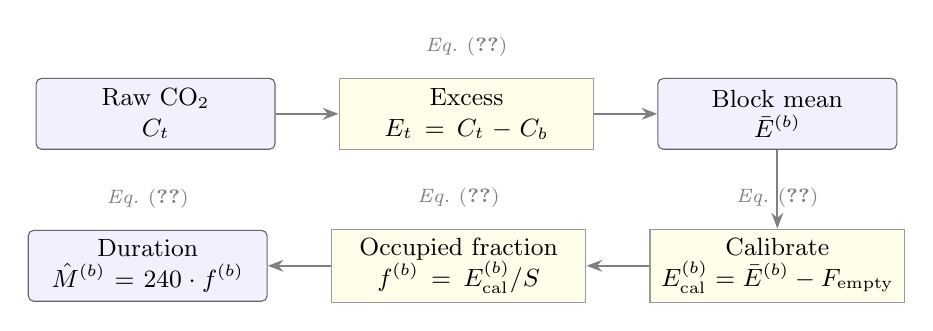
\begin{tikzpicture}[
        node distance=0.5cm and 0.8cm,
        proc/.style={rectangle, draw=black!60, fill=blue!6, text width=2.8cm, minimum height=0.9cm, align=center, rounded corners=2pt, font=\small},
        math/.style={rectangle, draw=black!40, fill=yellow!8, text width=3.0cm, minimum height=0.9cm, align=center, font=\small},
        arrow/.style={-{Stealth[length=2mm]}, thick, draw=black!50},
    ]
        % Row 1
        \node[proc] (raw) {Raw CO\textsubscript{2}\\$C_t$};
        \node[math, right=0.8cm of raw] (excess) {Excess\\$E_t = C_t - C_b$};
        \node[proc, right=0.8cm of excess] (blockmean) {Block mean\\$\bar{E}^{(b)}$};

        % Row 2
        \node[math, below=1.0cm of blockmean] (cal) {Calibrate\\$E_\text{cal}^{(b)} = \bar{E}^{(b)} - F_\text{empty}$};
        \node[math, left=0.8cm of cal] (frac) {Occupied fraction\\$f^{(b)} = E_\text{cal}^{(b)} / S$};
        \node[proc, left=0.8cm of frac] (minutes) {Duration\\$\hat{M}^{(b)} = 240 \cdot f^{(b)}$};

        % Arrows
        \draw[arrow] (raw) -- (excess);
        \draw[arrow] (excess) -- (blockmean);
        \draw[arrow] (blockmean) -- (cal);
        \draw[arrow] (cal) -- (frac);
        \draw[arrow] (frac) -- (minutes);

        % Annotations
        \node[font=\scriptsize\itshape, text=black!50, above=0.15cm of excess] {Eq.~\eqref{eq:excess}};
        \node[font=\scriptsize\itshape, text=black!50, above=0.15cm of cal] {Eq.~\eqref{eq:cal_excess}};
        \node[font=\scriptsize\itshape, text=black!50, above=0.15cm of frac] {Eq.~\eqref{eq:occ_fraction}};
        \node[font=\scriptsize\itshape, text=black!50, above=0.15cm of minutes] {Eq.~\eqref{eq:minutes}};
    \end{tikzpicture}
    \caption{Estimation pipeline for a single four-hour block. Raw CO\textsubscript{2} is converted to excess above baseline, averaged over the block, calibrated against the per-sensor empty-room floor, normalized by the blended scale $S$, and converted to occupied minutes.}
    \label{fig:estimation_pipeline}
\end{figure}

\begin{figure}[htbp]
    \centering
    \includegraphics[width=\textwidth]{figures/fig11_model_physics_illustration.pdf}
    \caption{Illustration of the CO\textsubscript{2} dynamics model and block-level estimation. The top panel shows the CO\textsubscript{2} time series with excess above baseline. The estimation procedure computes mean excess per block, subtracts the per-sensor empty-room floor, and normalizes by the blended scale $S$ to obtain occupied fraction.}
    \label{fig:physics_illustration}
\end{figure}

% -----------------------------------------------------------------------------
\subsection{Monte Carlo uncertainty quantification}
\label{sec:mc_uncertainty}
% -----------------------------------------------------------------------------

Uncertainty in the duration estimates arises primarily from parameter estimation error (in $\hat{\phi}$, $\hat{g}$, and $F_\text{empty}$) and model misspecification. We propagate parameter uncertainty using Monte Carlo simulation with $N_\text{MC} = 200$ samples, treating the observed block means as fixed data (conditional inference).

For each Monte Carlo sample $s = 1, \ldots, N_\text{MC}$:
\begin{enumerate}
    \item Draw perturbed parameters:
    \begin{align}
        \phi^{(s)} &\sim \text{TruncNormal}\!\left(\hat{\phi}, \; \text{SE}(\hat{\phi}), \; [\phi_\text{min}, \phi_\text{max}]\right) \\
        g^{(s)} &\sim \text{TruncNormal}\!\left(\hat{g}, \; \text{SE}(\hat{g}), \; [g_\text{min}, g_\text{max}]\right) \\
        F^{(s)} &\sim \text{TruncNormal}\!\left(F_\text{empty}, \; 0.5 \, s_\text{empty}, \; [0, \infty)\right)
    \end{align}
    \item Compute perturbed normalization scale $S^{(s)}$ using Eq.~\eqref{eq:scale} with $\hat{g} \to g^{(s)}$ and $\hat{\phi} \to \phi^{(s)}$.
    \item Compute estimated minutes $\hat{M}^{(b,s)}$ using Eqs.~\eqref{eq:cal_excess}--\eqref{eq:minutes} with perturbed quantities and the observed (fixed) block-mean excess $\bar{E}^{(b)}$.
\end{enumerate}

No separate observation-noise term is added to the block mean.  The original formulation used $\eta \sim \mathcal{N}(0, \hat{\sigma}_\varepsilon^2 / n_b)$, which assumes independent observations within a block.  Because the AR(1) autocorrelation ($\hat{\phi} \approx 0.995$) severely violates this assumption, the effective sample size is far smaller than $n_b$ and the $\sigma/\sqrt{n}$ formula underestimates block-mean variance.  Rather than substitute an ad-hoc empirical scale, we treat the observed block mean as fixed data (conditional inference) and let the parameter perturbation ($\phi$, $g$, $F_\text{empty}$) capture the dominant uncertainty sources.

The point estimate for each block is taken as the median across Monte Carlo samples ($\hat{M}^{(b)}_\text{p50}$), and the 80\% credible interval is $[\hat{M}^{(b)}_\text{p10}, \; \hat{M}^{(b)}_\text{p90}]$. The uncertainty width is defined as:
\begin{equation}
    W^{(b)} = \hat{M}^{(b)}_\text{p90} - \hat{M}^{(b)}_\text{p10}
    \label{eq:uncertainty_width}
\end{equation}

Blocks are classified as ``high confidence'' when $W^{(b)} \leq \SI{30}{min}$ (i.e., the 80\% credible interval spans no more than one eighth of the block duration).

% -----------------------------------------------------------------------------
\subsection{Validation framework}
\label{sec:validation}
% -----------------------------------------------------------------------------

We evaluate the method using two tiers of assessment criteria, illustrated in Fig.~\ref{fig:validation_framework}. The first tier comprises two \emph{calibration diagnostics} (C1--C2) that were used to select the floor multiplier $k$ (Section~\ref{sec:block_estimation}) and therefore cannot serve as independent validation. The second tier comprises four \emph{independent evaluation criteria} (E1--E4) that test aspects of estimation quality not involved in any tuning decision. We additionally report two supplementary out-of-sample checks (C1-OOS, C2-OOS) with relaxed thresholds.

\begin{figure}[htbp]
    \centering
    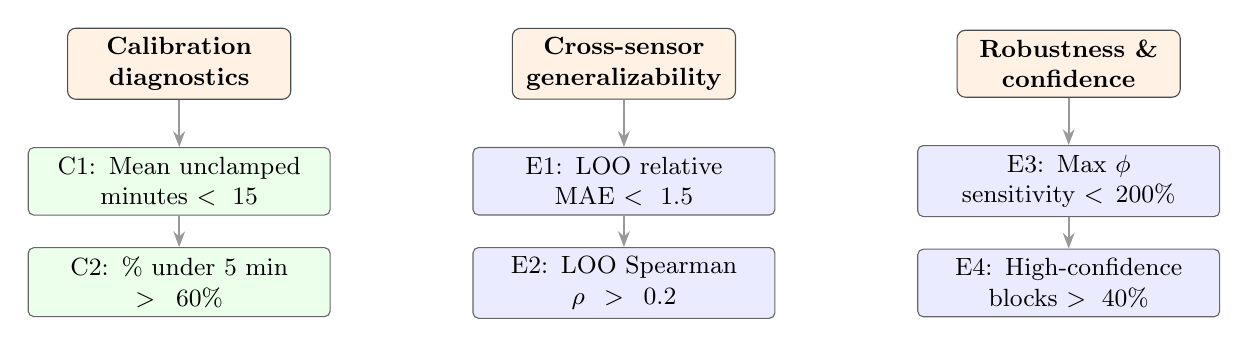
\begin{tikzpicture}[
        node distance=0.4cm and 0.6cm,
        test/.style={rectangle, draw=black!60, fill=blue!8, text width=3.6cm, minimum height=0.85cm, align=center, rounded corners=2pt, font=\small},
        cal/.style={rectangle, draw=black!60, fill=green!8, text width=3.6cm, minimum height=0.85cm, align=center, rounded corners=2pt, font=\small},
        cat/.style={rectangle, draw=black!70, fill=orange!10, text width=2.6cm, minimum height=0.85cm, align=center, rounded corners=3pt, font=\small\bfseries},
        arrow/.style={-{Stealth[length=2mm]}, thick, draw=black!40},
    ]
        % Categories
        \node[cat] (calib) {Calibration\\diagnostics};
        \node[cat, right=2.8cm of calib] (general) {Cross-sensor\\generalizability};
        \node[cat, right=2.8cm of general] (robust) {Robustness \&\\confidence};

        % Tests under Calibration
        \node[cal, below=0.6cm of calib] (t1) {C1: Mean unclamped\\minutes $< 15$};
        \node[cal, below=0.4cm of t1] (t2) {C2: \% under 5 min\\$> 60\%$};

        % Tests under Generalizability
        \node[test, below=0.6cm of general] (t3) {E1: LOO relative\\MAE $< 1.5$};
        \node[test, below=0.4cm of t3] (t4) {E2: LOO Spearman\\$\rho > 0.2$};

        % Tests under Robustness
        \node[test, below=0.6cm of robust] (t5) {E3: Max $\phi$\\sensitivity $< 200\%$};
        \node[test, below=0.4cm of t5] (t6) {E4: High-confidence\\blocks $> 40\%$};

        % Arrows
        \draw[arrow] (calib) -- (t1);
        \draw[arrow] (t1) -- (t2);
        \draw[arrow] (general) -- (t3);
        \draw[arrow] (t3) -- (t4);
        \draw[arrow] (robust) -- (t5);
        \draw[arrow] (t5) -- (t6);
    \end{tikzpicture}
    \caption{Validation framework organized into calibration diagnostics (C1--C2, green) and independent evaluation criteria (E1--E4, blue). C1--C2 were used to select the floor multiplier $k$ and are therefore in-sample by construction. E1--E4 test cross-sensor generalizability, parameter robustness, and uncertainty informativeness independently of the calibration.}
    \label{fig:validation_framework}
\end{figure}

\subsubsection{Calibration diagnostics (C1--C2)}

These criteria were used to select the floor multiplier $k$ (Section~\ref{sec:block_estimation}) and are therefore met by construction. They verify that the selected $k$ achieves adequate empty-room specificity but do not constitute independent validation.

\begin{enumerate}
    \item[C1.] \textbf{Label = 0 mean unclamped minutes} (${<}\SI{15}{min}$): For blocks where the occupant self-reported absence for the entire four-hour period, the mean estimated duration should be small. ``Unclamped'' means estimates are computed using the same model without forcing label = 0 blocks to zero.

    \item[C2.] \textbf{Label = 0 \% under \SI{5}{min}} (${>}60\%$): The majority of known-empty blocks should produce near-zero duration estimates. This is a stronger test than the mean criterion, requiring consistent (not just average) recognition of empty conditions.
\end{enumerate}

\subsubsection{Independent evaluation criteria (E1--E4)}

These criteria were not involved in any tuning decision and provide independent assessment of estimation quality.

\begin{enumerate}
    \item[E1.] \textbf{Leave-one-sensor-out (LOO) mean relative MAE} (${<}1.5$): For each sensor, we estimate block durations using physics parameters ($\hat{\phi}$, $\hat{g}$) from the \emph{remaining} sensors (cross-sensor median). The mean absolute error relative to sensor-specific estimates should be moderate, demonstrating that the method generalizes across rooms with different ventilation characteristics.

    \item[E2.] \textbf{LOO mean Spearman rank correlation} (${>}0.2$): The rank ordering of block durations should be preserved when using cross-sensor parameters. This tests whether the method captures \emph{relative} occupancy patterns even when absolute calibration differs.

    \item[E3.] \textbf{Max $\phi$ sensitivity (\% change)} (${<}200\%$): Varying the decay parameter across the range $[0.90, 0.99]$ should produce smooth, bounded changes in mean duration estimates. This tests robustness to the most uncertain physical parameter.

    \item[E4.] \textbf{\% blocks with high confidence} (${>}40\%$): A substantial fraction of occupied blocks should have tight uncertainty bounds (80\% CI width ${\leq}\SI{30}{min}$). This tests whether the method provides actionable uncertainty information.
\end{enumerate}

\subsubsection{Out-of-sample temporal split}

Calibration diagnostics C1 and C2 use the same empty blocks both to fit the empty-room floor $F_\text{empty}$ and to evaluate it, creating an in-sample bias risk.  To verify that the calibration generalizes to unseen days, we repeat C1--C2 using a temporal split: for each sensor, empty blocks are sorted chronologically, the first 70\% are used to fit $F_\text{empty}$, and the remaining 30\% are evaluated with that floor.  The out-of-sample criteria are relaxed to C1-OOS~$< \SI{20}{min}$ and C2-OOS~$> 50\%$.

\subsubsection{Baseline comparators}

To demonstrate that the block-excess approach adds value beyond simpler heuristics, we compare against two baseline methods applied to the same sensor data:
\begin{itemize}
    \item \textbf{Threshold method}: For each block, count the number of minutes where excess CO\textsubscript{2} exceeds a fixed threshold (50, 100, or \SI{200}{ppm}).
    \item \textbf{Slope method}: For each block, count the number of minutes where CO\textsubscript{2} concentration is rising (positive first difference).
\end{itemize}
Each baseline is evaluated on the same C1 and C2 criteria as the block-excess estimator.

\subsubsection{Semisynthetic validation}
\label{sec:semisynthetic_methods}

Because no ground-truth occupied minutes are available, we construct a semisynthetic validation by injecting known synthetic occupancy patterns into real empty-room CO\textsubscript{2} segments.  The procedure is:
\begin{enumerate}
    \item Select contiguous truly-empty blocks ($\geq 200$ minutes of data, mean excess $< \SI{20}{ppm}$, room-level empty).
    \item Define synthetic occupancy scenarios: continuous presence for 30, 60, 120, 180, or 240 minutes, fragmented patterns (4$\times$30~min with gaps, 2$\times$60~min with gap), and model-mismatch stress tests (see below).
    \item Inject a \emph{deterministic} synthetic excess into the real empty data using the sensor's fitted $\hat{\phi}$ and $\hat{g}$:
    \begin{equation}
        E_t^\text{inj} = \hat{\phi} \, E_{t-1}^\text{inj} + \hat{g} \cdot O_t^\text{synth}
    \end{equation}
    The injected component contains no added noise because the real empty segment already carries realistic innovations and building transients; adding noise would double-count.  The synthetic CO\textsubscript{2} is then $C_t^\text{synth} = C_t^\text{empty} + E_t^\text{inj}$.
    \item For stress tests, injection uses parameters that differ from those assumed by the estimator, testing robustness to model mismatch: generation-rate mismatch ($\hat{g}' = 0.7\hat{g}$ and $1.3\hat{g}$), decay-rate drift ($\hat{\phi}' = \hat{\phi} + 0.005$), a $+\SI{30}{ppm}$ baseline shift, and extra innovation noise ($\eta_t \sim \mathcal{N}(0, \hat{\sigma}_\varepsilon^2)$ added to the injected component).
    \item Run the block-excess estimator on the synthetic data using the same $F_\text{empty}$ and scale~$S$ as the real estimation.
    \item Compute MAE, bias, and error distributions across scenarios.
\end{enumerate}

% =============================================================================
\section{Results}
\label{sec:results}
% =============================================================================

% -----------------------------------------------------------------------------
\subsection{Sensor physics parameters}
\label{sec:sensor_params}
% -----------------------------------------------------------------------------

Table~\ref{tab:sensor_params} presents the fitted AR(1) model parameters for each of the 12 sensors. The decay parameter $\hat{\phi}$ ranges from 0.970 to 0.995, corresponding to effective air exchange rates of 0.005 to 0.030 per minute (\SIrange{0.3}{1.8}{ACH}). The CO\textsubscript{2} generation rate $\hat{g}$ ranges from \SIrange{5.4}{60.0}{ppm/min}, reflecting differences in room size, ventilation configuration, and occupant metabolic characteristics. Baseline CO\textsubscript{2} concentrations range from \SIrange{405.8}{542.0}{ppm}, with most sensors near the typical outdoor level of ${\sim}\SI{410}{ppm}$ and one sensor (22168412) showing an elevated baseline of \SI{542.0}{ppm}, likely reflecting reduced ventilation or proximity to a CO\textsubscript{2} source. Sensor~20233681 has zero valid decay observations and uses the prior default for $\hat{\phi}$ (flagged in Table~\ref{tab:sensor_params}).

\begin{table}[htbp]
\centering
\caption{Fitted AR(1) model parameters for each sensor. $C_b$: baseline CO\textsubscript{2} concentration; $\hat{\phi}$: decay parameter; $\hat{g}$: generation rate; $\hat{\sigma}_\varepsilon$: innovation noise standard deviation; $n_\text{decay}$: number of valid decay observations; Fallback: parameters using prior defaults instead of sensor-specific fits.}
\label{tab:sensor_params}
\small
\begin{tabular}{lccccccc}
\toprule
Sensor ID & Room type & $C_b$ (ppm) & $\hat{\phi}$ & $\hat{g}$ (ppm/min) & $\hat{\sigma}_\varepsilon$ (ppm) & $n_\text{decay}$ & Fallback \\
\midrule
20233647 & Single & 443.7 & 0.992 & 18.9 & 17.1 & 693 & none \\
20233665 & Single & 481.4 & 0.995 & 30.5 & 31.6 & 1658 & none \\
20233681 & Single & 409.0 & 0.970 & 60.0 & 35.0 & 0 & $\phi$ \\
20233685 & Single & 457.1 & 0.991 & 14.5 & 7.3 & 2081 & none \\
20251591 & Single & 405.9 & 0.987 & 11.9 & 21.0 & 1897 & none \\
22165976 & Shared & 405.8 & 0.995 & 16.3 & 9.0 & 2880 & none \\
22165978 & Single & 477.3 & 0.994 & 5.4 & 9.7 & 2974 & none \\
22165989 & Single & 419.3 & 0.995 & 22.8 & 15.1 & 1200 & none \\
22165990 & Single & 412.6 & 0.970 & 26.2 & 5.7 & 50 & none \\
22165993 & Single & 475.6 & 0.987 & 30.2 & 11.9 & 240 & none \\
22165994 & Shared & 407.4 & 0.987 & 7.7 & 10.1 & 353 & none \\
22168412 & Shared & 542.0 & 0.984 & 19.2 & 22.4 & 240 & none \\
\bottomrule
\end{tabular}
\end{table}

Fig.~\ref{fig:sensor_params} visualizes the distribution of sensor parameters across rooms. The strong clustering of $\hat{\phi}$ near 0.995 reflects the tight, well-insulated construction typical of modern dormitory buildings.

\begin{figure}[htbp]
    \centering
    \includegraphics[width=0.9\textwidth]{figures/fig04_sensor_parameters.pdf}
    \caption{Distribution of fitted sensor physics parameters across the 12 monitored rooms.}
    \label{fig:sensor_params}
\end{figure}

% -----------------------------------------------------------------------------
\subsection{Block-level duration estimates}
\label{sec:block_results}
% -----------------------------------------------------------------------------

Table~\ref{tab:block_summary} summarizes the estimated occupancy duration by occupancy label. For known-absent blocks (label = 0), the unclamped estimates average \SI{14.9}{min} with a block-level median of \SI{0.0}{min}, matching the C1 calibration diagnostic exactly (both computed from the same unclamped re-estimation). Overall, 85.4\% of absent blocks estimate under \SI{5}{min}, confirming that the method correctly identifies empty rooms in the large majority of cases. For downstream use, label = 0 blocks are clamped to zero. For known-present blocks (label = 1), the mean estimated duration is \SI{69.4}{min} with a median of \SI{0.0}{min}; 47\% of occupied blocks produce nonzero estimates. This right-skewed distribution reflects the conservative empty-room floor and the nature of four-hour block labeling: many blocks labeled ``present'' involve brief visits that do not elevate CO\textsubscript{2} above the per-sensor floor, while a smaller number of blocks show sustained presence with correspondingly higher duration estimates.

\begin{table}[htbp]
\centering
\caption{Block-level duration estimates by occupancy label. Label = 0 values are \emph{unclamped} (not forced to zero); for downstream use they are clamped. All values in minutes (out of 240-minute blocks). $n$: number of blocks; uncertainty refers to the width of the 80\% credible interval.}
\label{tab:block_summary}
\begin{tabular}{lccccccc}
\toprule
Label & $n$ & Mean & Median & SD & Min & Max & Mean uncertainty \\
\midrule
0 (absent, unclamped) & 239 & 14.9 & 0.0 & 47.7 & 0.0 & 240.0 & 28.9 \\
1 (present) & 535 & 69.4 & 0.0 & 90.1 & 0.0 & 240.0 & 61.2 \\
\bottomrule
\end{tabular}
\end{table}

The right-skewed distribution of label = 1 estimates (Fig.~\ref{fig:histogram}) is consistent with the nature of four-hour block labeling: a ``present'' label indicates the occupant was in the room for \emph{at least some portion} of the block. Many blocks labeled as present may correspond to brief entries (returning to retrieve an item, checking in briefly) that produce modest CO\textsubscript{2} elevation above the empty-room floor, while extended study or sleep sessions produce sustained elevation and correspondingly higher duration estimates.

\begin{figure}[htbp]
    \centering
    \includegraphics[width=0.9\textwidth]{figures/fig01_histogram_by_label.pdf}
    \caption{Distribution of estimated occupancy duration by label. Label = 0 blocks cluster at zero minutes. Label = 1 blocks show a right-skewed distribution with many low-duration blocks and a tail extending to 240 minutes.}
    \label{fig:histogram}
\end{figure}

% -----------------------------------------------------------------------------
\subsection{Time-of-day patterns}
\label{sec:time_of_day}
% -----------------------------------------------------------------------------

Fig.~\ref{fig:time_of_day} shows the estimated occupancy duration by time-of-day block. As expected for a university dormitory population, occupancy is highest during the overnight block (22:00--02:00) when students are sleeping and lowest during the midday blocks (10:00--14:00 and 14:00--18:00) when students are attending classes and engaged in campus activities.

\begin{figure}[htbp]
    \centering
    \includegraphics[width=0.9\textwidth]{figures/fig02_time_of_day_pattern.pdf}
    \caption{Estimated occupancy duration by time-of-day block. Error bars show the interquartile range across subjects. The overnight block (22:00--02:00) shows the highest occupancy, while midday blocks show the lowest, consistent with university student schedules.}
    \label{fig:time_of_day}
\end{figure}

% -----------------------------------------------------------------------------
\subsection{CO\textsubscript{2} trace examples}
\label{sec:trace_examples}
% -----------------------------------------------------------------------------

Fig.~\ref{fig:traces} presents representative CO\textsubscript{2} time series for selected sensors, illustrating the relationship between CO\textsubscript{2} dynamics and occupancy patterns. The traces demonstrate the characteristic rise during occupancy (CO\textsubscript{2} generation from breathing) and exponential decay after departure (ventilation removing excess CO\textsubscript{2}). The variation in baseline levels, peak concentrations, and decay rates across sensors reflects the heterogeneity of room ventilation and occupant behavior captured by the per-sensor parameter fitting.

\begin{figure}[htbp]
    \centering
    \includegraphics[width=\textwidth]{figures/fig03_co2_trace_examples.pdf}
    \caption{Representative CO\textsubscript{2} time series for selected sensors. Shaded regions indicate four-hour blocks labeled as present (label = 1). The exponential decay after occupancy departure and the rise during presence illustrate the AR(1) dynamics captured by the model.}
    \label{fig:traces}
\end{figure}

% -----------------------------------------------------------------------------
\subsection{Validation results}
\label{sec:validation_results}
% -----------------------------------------------------------------------------

Table~\ref{tab:validation} presents the validation results. Both calibration diagnostics (C1--C2) are met by construction (these criteria were used to select $k$). All four independent evaluation criteria (E1--E4) are satisfied. The out-of-sample temporal split test (C1-OOS) exceeds its criterion, indicating that the empty-room calibration benefits from the full dataset. These results are discussed in Section~\ref{sec:discussion}.

\begin{table}[htbp]
\centering
\caption{Validation results. Calibration diagnostics (C1--C2) are met by construction; all four independent evaluation criteria (E1--E4) are satisfied. Out-of-sample C1-OOS exceeds its criterion.}
\label{tab:validation}
\begin{tabular}{llcccp{5.0cm}}
\toprule
Tier & Test & Value & Criterion & Pass? & Interpretation \\
\midrule
\multicolumn{6}{l}{\emph{Calibration diagnostics (used to select $k$; in-sample by construction)}} \\
& C1: Label = 0 mean unclamped min & 14.9 & ${<}15$ & YES & Empty-room floor correctly calibrated \\
& C2: Label = 0 \% under 5~min & 85.4\% & ${>}60\%$ & YES & Majority of absent blocks near zero \\
\midrule
\multicolumn{6}{l}{\emph{Out-of-sample temporal split}} \\
& C1-OOS: mean unclamped min & 46.0 & ${<}20$ & NO & Calibration degrades with limited data \\
& C2-OOS: \% under 5~min & 61.4\% & ${>}50\%$ & YES & Majority of held-out absent blocks near zero \\
\midrule
\multicolumn{6}{l}{\emph{Independent evaluation criteria}} \\
& E1: LOO mean relative MAE & 1.11 & ${<}1.5$ & YES & Cross-sensor parameters within 150\% \\
& E2: LOO mean Spearman $\rho$ & 0.313 & ${>}0.2$ & YES & Rank ordering preserved cross-sensor \\
& E3: Max $\phi$ sensitivity (\%) & 30.7\% & ${<}200\%$ & YES & Smooth response to decay parameter \\
& E4: \% blocks high confidence & 50.7\% & ${>}40\%$ & YES & About half of estimates have tight uncertainty \\
\bottomrule
\end{tabular}
\end{table}

\subsubsection{Label = 0 sanity check}

The mean unclamped estimated duration for the 239~known-empty blocks is \SI{14.9}{min}, below the \SI{15}{min} criterion. Of these blocks, 85.4\% estimate less than \SI{5}{min} of occupancy (82.4\% estimate exactly zero), with a heavy concentration near zero and a tail of larger residual-duration false positives for the remaining 14.6\% of blocks (Fig.~\ref{fig:label0_validation}).

\begin{figure}[htbp]
    \centering
    \includegraphics[width=0.8\textwidth]{figures/fig06_validation_label0.pdf}
    \caption{Distribution of unclamped estimated duration for known-empty (label = 0) blocks. The majority cluster at or near zero, with a tail of false positives from blocks where residual CO\textsubscript{2} from prior occupancy exceeds the per-sensor empty-room floor.}
    \label{fig:label0_validation}
\end{figure}

The 14.6\% of empty blocks that estimate above \SI{5}{min} represent cases where residual CO\textsubscript{2} from occupancy in a preceding block has not fully decayed during the current block, producing excess CO\textsubscript{2} that exceeds the per-sensor empty-room floor. This is physically expected given the long decay time constants ($\tau = 1/(1-\phi) \approx \SIrange{33}{200}{min}$) and is captured by the uncertainty bounds.

\subsubsection{Leave-one-sensor-out cross-validation}

Table~\ref{tab:loo} presents the leave-one-sensor-out results. For each sensor, block durations are estimated using the median $\hat{\phi}$ and median $\hat{g}$ from the remaining 11 sensors (cross-sensor parameters). The mean absolute error relative to sensor-specific estimates is 1.11 (criterion: ${<}1.5$), and the mean Spearman rank correlation is 0.313 (criterion: ${>}0.2$).

\begin{table}[htbp]
\centering
\caption{Leave-one-sensor-out cross-validation results. $\hat{\phi}_\text{own}$, $\hat{g}_\text{own}$: sensor-specific parameters; $\hat{\phi}_\text{cross}$, $\hat{g}_\text{cross}$: median of remaining sensors; MAE: mean absolute error (minutes); Rel.\ MAE: relative MAE (ratio); $\rho$: Spearman rank correlation between own and cross estimates.}
\label{tab:loo}
\small
\begin{tabular}{lccccccc}
\toprule
Sensor ID & Room & $\hat{\phi}_\text{own}$ & $\hat{g}_\text{own}$ & $\hat{g}_\text{cross}$ & MAE & Rel.\ MAE & $\rho$ \\
\midrule
20233647 & Single & 0.992 & 18.9 & 19.2 & 51.9 & 1.14 & 0.62 \\
20233665 & Single & 0.995 & 30.5 & 18.9 & 54.9 & 2.52 & 0.56 \\
20233681 & Single & 0.970 & 60.0 & 18.9 & 67.7 & 0.37 & 0.09 \\
20233685 & Single & 0.991 & 14.5 & 19.2 & 80.1 & 0.61 & 0.07 \\
20251591 & Single & 0.987 & 11.9 & 19.2 & 57.4 & 0.74 & 0.03 \\
22165976 & Shared & 0.995 & 16.3 & 19.2 & 82.3 & 0.94 & 0.23 \\
22165978 & Single & 0.994 & 5.4 & 19.2 & 8.7 & 1.27 & 0.76 \\
22165989 & Single & 0.995 & 22.8 & 18.9 & 0.6 & 0.57 & 0.00 \\
22165990 & Single & 0.970 & 26.2 & 18.9 & 79.4 & 0.77 & 0.05 \\
22165993 & Single & 0.986 & 30.2 & 18.9 & 92.8 & 1.58 & 0.26 \\
22165994 & Shared & 0.987 & 7.7 & 19.2 & 4.3 & 1.16 & 0.86 \\
22168412 & Shared & 0.984 & 19.2 & 18.9 & 58.5 & 1.62 & 0.23 \\
\midrule
\multicolumn{5}{l}{Mean} & 53.2 & 1.11 & 0.313 \\
\bottomrule
\end{tabular}
\end{table}

Cross-sensor performance varies considerably across rooms. Several sensors retain moderate-to-strong rank agreement under cross-sensor parameters (e.g., 22165994 with $\rho = 0.86$ and 22165978 with $\rho = 0.76$), while others show weak agreement (e.g., 22165989 with $\rho = 0.00$ and 20251591 with $\rho = 0.03$). This spread reflects ventilation heterogeneity and the fact that many blocks lie near the empty-room floor, where small calibration differences determine whether a block estimates as nonzero. The heterogeneity motivates the per-sensor calibration approach.

\subsubsection{Sensitivity analysis}

Fig.~\ref{fig:sensitivity_phi} shows the sensitivity of estimated duration to the decay parameter $\phi$ across the range $[0.90, 0.99]$. The mean estimated duration varies from \SI{55.4}{min} ($\phi = 0.99$) to \SI{100.0}{min} ($\phi = 0.90$), compared to \SI{80.0}{min} at the default $\phi = 0.97$. The maximum percentage change relative to the default is 30.7\% (at $\phi = 0.99$)---well within the 200\% criterion. The monotonic decrease with increasing $\phi$ is physically intuitive: higher $\phi$ (slower decay) produces larger normalization scale, so a given observed excess corresponds to a smaller occupied fraction.

\begin{figure}[htbp]
    \centering
    \includegraphics[width=0.8\textwidth]{figures/fig07_sensitivity_phi.pdf}
    \caption{Sensitivity of estimated occupancy duration to the decay parameter $\phi$. Mean and median estimated duration (across all label = 1 blocks) are shown for each $\phi$ value. The smooth, monotonic response indicates robust behavior without discontinuities or instabilities.}
    \label{fig:sensitivity_phi}
\end{figure}

Fig.~\ref{fig:sensitivity_gen} shows the sensitivity to the generation rate multiplier. Scaling the generation rate from $0.5\times$ to $2.0\times$ produces a monotonic decrease in estimated duration from \SI{88.9}{min} to \SI{52.2}{min}, consistent with the physics: higher generation rates produce more CO\textsubscript{2} per minute of occupancy, so a given observed excess corresponds to fewer occupied minutes.

\begin{figure}[htbp]
    \centering
    \includegraphics[width=0.8\textwidth]{figures/fig08_sensitivity_generation.pdf}
    \caption{Sensitivity of estimated occupancy duration to the generation rate multiplier. Multipliers of $0.5\times$ to $2.0\times$ are applied to each sensor's fitted $\hat{g}$.}
    \label{fig:sensitivity_gen}
\end{figure}

% -----------------------------------------------------------------------------
\subsection{Uncertainty analysis}
\label{sec:uncertainty_results}
% -----------------------------------------------------------------------------

Fig.~\ref{fig:uncertainty} shows the distribution of uncertainty widths (80\% credible interval spans) across all occupied blocks. The mean uncertainty width is \SI{61.2}{min}, and 50.7\% of occupied blocks achieve ``high confidence'' status (width ${\leq}\SI{30}{min}$). High-confidence blocks tend to be those with either very low or very high mean excess CO\textsubscript{2}: blocks near the empty-room floor produce tight estimates near zero, while blocks with very high excess produce tight estimates near the block maximum. Intermediate excess levels, where the calibrated signal is comparable to the parameter uncertainty, naturally produce wider confidence intervals.

\begin{figure}[htbp]
    \centering
    \includegraphics[width=0.8\textwidth]{figures/fig05_uncertainty_analysis.pdf}
    \caption{Uncertainty analysis of block-level duration estimates. Distribution of 80\% credible interval widths across all occupied (label = 1) blocks.}
    \label{fig:uncertainty}
\end{figure}

% -----------------------------------------------------------------------------
\subsection{Individual subject profiles}
\label{sec:individual}
% -----------------------------------------------------------------------------

Table~\ref{tab:subject_summary} reports participant-level summaries constructed from \emph{room-level} CO\textsubscript{2}-based duration estimates for the 18 participants in 9 single-occupancy rooms. Because each sensor measures a shared room environment, the CO\textsubscript{2}-based duration estimate for a given block is the same for all participants associated with that sensor. Participant-level totals therefore differ only because they are aggregated over different subsets of blocks based on each participant's self-reported presence (i.e., schedule-weighting), and should not be interpreted as CO\textsubscript{2}-based disaggregation of individuals. For example, participants 324 and 325 (sensor 20233665) average \SI{52}{} and \SI{104}{min/day} respectively because they reported being present for different blocks. Participants with identical survey responses produce identical estimates (73/95, 506/507). The estimated mean daily room occupancy ranges from \SI{0.0}{min/day} (participants 506, 507) to \SI{985.5}{min/day} (participant 96).

\begin{table}[htbp]
\centering
\caption{Participant-level occupancy summary for single-occupancy rooms (18 participants, 9 sensors). Each sensor monitors one room; two study participants per room provided independent self-reported presence schedules. The CO\textsubscript{2}-based duration estimate is computed at the room level, so differences between participants on the same sensor arise solely from different self-reported presence patterns, not from distinct CO\textsubscript{2} signals. Mean, median, and standard deviation of daily estimated room occupancy (minutes per day). P10 and P90 are the mean daily 10th and 90th percentile estimates from the Monte Carlo uncertainty propagation.}
\label{tab:subject_summary}
\small
\begin{tabular}{lcccccccc}
\toprule
Subject & Sensor & Days & Mean & Median & SD & P10 & P90 \\
\midrule
96 & 20233681 & 7 & 985.5 & 1046.1 & 353.9 & 374.5 & 1199.3 \\
151 & 20233681 & 7 & 937.8 & 814.1 & 230.7 & 346.7 & 1191.8 \\
474 & 20233685 & 6 & 539.4 & 591.3 & 362.3 & 456.6 & 640.1 \\
471 & 22165990 & 6 & 449.1 & 500.3 & 202.1 & 305.2 & 626.2 \\
508 & 20233685 & 4 & 381.5 & 361.4 & 77.0 & 333.0 & 442.8 \\
472 & 22165990 & 6 & 359.2 & 439.5 & 246.3 & 252.1 & 471.9 \\
37 & 22165993 & 6 & 264.6 & 289.2 & 244.2 & 157.7 & 426.0 \\
38 & 22165993 & 6 & 264.6 & 289.2 & 244.2 & 157.7 & 395.3 \\
117 & 20233647 & 7 & 205.7 & 0.0 & 351.3 & 183.4 & 224.6 \\
154 & 20233647 & 7 & 188.7 & 0.0 & 338.6 & 152.4 & 235.3 \\
46 & 20251591 & 7 & 148.0 & 91.5 & 168.2 & 96.0 & 218.2 \\
42 & 20251591 & 1 & 48.9 & 48.9 & --- & 0.0 & 99.5 \\
325 & 20233665 & 6 & 104.2 & 0.0 & 161.6 & 19.6 & 230.6 \\
324 & 20233665 & 6 & 52.1 & 0.0 & 122.9 & 7.1 & 179.2 \\
73 & 22165978 & 6 & 13.7 & 0.0 & 33.6 & 2.3 & 25.0 \\
95 & 22165978 & 6 & 13.7 & 0.0 & 33.6 & 2.3 & 25.0 \\
506 & 22165989 & 6 & 0.0 & 0.0 & 0.0 & 0.0 & 38.3 \\
507 & 22165989 & 6 & 0.0 & 0.0 & 0.0 & 0.0 & 38.3 \\
\bottomrule
\end{tabular}
\end{table}

Table~\ref{tab:shared_room_summary} presents supplementary room-level results for the 3 shared rooms (6 subjects). Because the CO\textsubscript{2} sensor cannot distinguish individual occupants, these estimates reflect \emph{room-level} occupancy rather than per-person duration and are presented by sensor rather than by subject.

\begin{table}[htbp]
\centering
\caption{Room-level occupancy for shared rooms (3 sensors, 6 subjects). Values reflect combined room occupancy and cannot be attributed to individual occupants.}
\label{tab:shared_room_summary}
\small
\begin{tabular}{lcccccc}
\toprule
Sensor & Subjects & Days & Mean & Median & P10 & P90 \\
\midrule
22168412 & 132, 133 & 6 & 305.1 & 289.5 & 152.2 & 472.8 \\
22165976 & 75, 76 & 6 & 173.0 & 85.5 & 71.4 & 308.9 \\
22165994 & 399, 400 & 7 & 13.8 & 0.0 & 0.0 & 120.0 \\
\bottomrule
\end{tabular}
\end{table}

Fig.~\ref{fig:individual_profiles} visualizes the daily occupancy profiles for selected subjects, illustrating the diversity of temporal patterns captured by the method.

\begin{figure}[htbp]
    \centering
    \includegraphics[width=\textwidth]{figures/fig10_individual_profiles.pdf}
    \caption{Individual subject daily occupancy profiles for selected subjects. Each bar represents estimated room occupancy for one day, with error bars showing the 80\% credible interval. The diversity of patterns reflects different student lifestyles, from near-full-time room dwellers (top) to rarely present occupants (bottom).}
    \label{fig:individual_profiles}
\end{figure}

% -----------------------------------------------------------------------------
\subsection{Shared vs.\ single-occupancy rooms}
\label{sec:shared_vs_single}
% -----------------------------------------------------------------------------

Table~\ref{tab:shared_vs_single} compares estimation results between shared and single-occupancy rooms. Single-occupancy rooms show higher mean estimated duration (\SI{78.6}{min} vs.\ \SI{43.0}{min}) and higher mean CO\textsubscript{2} concentrations (\SI{1637}{ppm} vs.\ \SI{1251}{ppm}). The lower duration estimates for shared rooms may reflect greater ventilation (more door openings with two occupants), measurement dilution (one sensor capturing a shared space), or genuinely lower per-person occupancy time in rooms with social dynamics.

\begin{table}[htbp]
\centering
\caption{Comparison of block-level estimates between shared and single-occupancy rooms (label = 1 blocks only).}
\label{tab:shared_vs_single}
\begin{tabular}{lcccccc}
\toprule
Room type & $n_\text{blocks}$ & Subjects & Mean (min) & Median (min) & SD (min) & Mean CO\textsubscript{2} (ppm) \\
\midrule
Shared & 138 & 6 & 43.0 & 0.0 & 71.9 & 1251 \\
Single & 397 & 18 & 78.6 & 5.8 & 94.1 & 1637 \\
\bottomrule
\end{tabular}
\end{table}

% -----------------------------------------------------------------------------
\subsection{Daily heatmap}
\label{sec:heatmap}
% -----------------------------------------------------------------------------

Fig.~\ref{fig:heatmap} presents a heatmap of estimated occupancy across subjects and days, providing a compact overview of the temporal patterns in the dataset. The heatmap reveals both consistent patterns (e.g., some subjects with regular nighttime occupancy) and sporadic patterns (e.g., subjects who are occasionally absent for extended periods), consistent with the variability of university student schedules.

\begin{figure}[htbp]
    \centering
    \includegraphics[width=\textwidth]{figures/fig12_daily_heatmap.pdf}
    \caption{Heatmap of estimated daily room occupancy (minutes) across subjects and days. Darker colors indicate higher estimated occupancy. Missing data (days without CO\textsubscript{2} records or occupancy labels) appear as gaps.}
    \label{fig:heatmap}
\end{figure}

% =============================================================================
\section{Discussion}
\label{sec:discussion}
% =============================================================================

% -----------------------------------------------------------------------------
\subsection{Out-of-sample empty-room calibration}
% -----------------------------------------------------------------------------

To verify that the empty-room floor $F_\text{empty}$ generalizes beyond the blocks used to fit it, we repeated the C1--C2 tests using a temporal split: the first 70\% of each sensor's empty blocks (chronologically) were used to fit $F_\text{empty}$, and the remaining 30\% were evaluated with that floor.  The out-of-sample results are reported alongside the in-sample results in Table~\ref{tab:validation}.  C2-OOS remains acceptable (61.4\% of held-out empty blocks under \SI{5}{min}), but C1-OOS increases substantially to \SI{46.0}{min}, indicating that the empty-room floor is not fully stationary across days.  This likely reflects day-to-day changes in residual CO\textsubscript{2} carryover (e.g., ventilation transients, atypical high-excess events, and changing occupancy patterns in adjacent blocks) that are not well captured when the calibration period is short.  In practice, longer or periodically refreshed calibration windows may be needed for stable empty-room specificity.

% -----------------------------------------------------------------------------
\subsection{Comparison with baseline methods}
% -----------------------------------------------------------------------------

Fig.~\ref{fig:baseline_comparison} compares the block-excess estimator against simpler baselines: threshold methods (counting minutes where excess CO\textsubscript{2} exceeds 50, 100, or \SI{200}{ppm}) and a slope method (counting minutes with rising CO\textsubscript{2}).  Because the floor multiplier $k$ was selected using the empty-room calibration diagnostics (C1--C2), the block-excess method is expected to achieve strong empty-room specificity by design.  The baseline comparators illustrate the trade-offs of fixed-threshold and slope heuristics: low thresholds inflate false positives in empty periods, high thresholds miss low-intensity occupancy, and the slope method is sensitive to noise.  In contrast, the block-excess approach provides a per-sensor calibrated floor and yields interpretable duration estimates under a unified physics-based normalization.

\begin{figure}[htbp]
    \centering
    \includegraphics[width=\textwidth]{figures/fig14_baseline_comparison.pdf}
    \caption{Comparison of duration estimation methods on empty-room specificity.  (a)~C1: mean estimated minutes for known-empty blocks (lower is better).  (b)~C2: percentage of empty blocks estimating under \SI{5}{min} (higher is better).  (c)~Mean estimated minutes for occupied blocks.  The block-excess method achieves the calibration targets for empty-room specificity; baselines illustrate the trade-offs of simpler heuristics.}
    \label{fig:baseline_comparison}
\end{figure}

% -----------------------------------------------------------------------------
\subsection{Semisynthetic validation}
% -----------------------------------------------------------------------------

Because no ground-truth occupied minutes are available, we constructed a semisynthetic validation by injecting known synthetic occupancy patterns into real empty-room CO\textsubscript{2} segments (see Section~\ref{sec:semisynthetic_methods}).  Fig.~\ref{fig:semisynthetic} shows the results and Table~\ref{tab:semisynthetic_summary} provides numeric accuracy by scenario.  Across continuous scenarios, the estimator shows systematic underestimation, with bias ranging from approximately $-25$~min (30--120~min cases) to $-53$~min for full-block (240~min) occupancy.  Fragmented patterns produce comparable absolute errors but tend toward more negative bias than continuous occupancy of equal total duration (e.g., frag\_4$\times$30 bias $= -48$~min vs.\ cont\_120 bias $= -24$~min), consistent with block-level averaging smoothing out short visits.  The model-mismatch stress tests show that estimation degrades gracefully under parameter perturbation: generation-rate mismatch ($\hat{g} \times 0.7$ and $\times 1.3$), decay-rate drift ($\hat{\phi} + 0.005$), baseline shifts ($+\SI{30}{ppm}$), and extra innovation noise all produce bounded degradation (MAE \SIrange{64}{115}{min} for a true duration of 120~min).

\begin{figure}[htbp]
    \centering
    \includegraphics[width=\textwidth]{figures/fig13_semisynthetic_validation.pdf}
    \caption{Semisynthetic validation results.  (a)~Scatter plot of estimated vs.\ true injected occupied minutes.  Continuous scenarios (circles) cluster closer to the identity line than fragmented scenarios (triangles).  (b)~Distribution of absolute estimation error by true duration level.}
    \label{fig:semisynthetic}
\end{figure}

% Semisynthetic numeric summary table — values from pipeline
\begin{table}[htbp]
\centering
\caption{Semisynthetic validation accuracy by scenario.  MAE: mean absolute error; Bias: mean signed error (positive = overestimation); P90: 90th percentile of absolute error.  All values in minutes.  Stress tests inject with parameters that differ from those used by the estimator.}
\label{tab:semisynthetic_summary}
\small
\begin{tabular}{llccccc}
\toprule
Group & Scenario & True min & $n$ & MAE & Bias & P90 \\
\midrule
Continuous & cont\_30  & 30  & 11 & 24.5 & $-24.5$ & 30.0 \\
Continuous & cont\_60  & 60  & 11 & 31.4 & $-27.6$ & 60.0 \\
Continuous & cont\_120 & 120 & 11 & 63.3 & $-24.0$ & 120.0 \\
Continuous & cont\_180 & 180 & 11 & 93.1 & $-33.5$ & 180.0 \\
Continuous & cont\_240 & 240 & 9 & 52.7 & $-52.7$ & 233.9 \\
\midrule
Fragmented & frag\_4x30 & 120 & 11 & 49.5 & $-48.1$ & 120.0 \\
Fragmented & frag\_2x60 & 120 & 11 & 50.9 & $-39.2$ & 120.0 \\
\midrule
Stress     & $g \times 0.7$  & 120 & 11 & 64.3 & $-64.3$ & 120.0 \\
Stress     & $g \times 1.3$  & 120 & 11 & 103.7 & $+16.4$ & 120.0 \\
Stress     & baseline   & 120 & 11 & 70.7 & $-16.6$ & 120.0 \\
Stress     & $\phi + 0.005$ & 120 & 11 & 115.1 & $+33.4$ & 120.0 \\
Stress     & extra noise     & 120 & 11 & 63.9 & $-22.6$ & 120.0 \\
\bottomrule
\end{tabular}
\end{table}

This validation is ``model-matched'' in the sense that both injection and estimation use the same AR(1) model form.  The stress tests partially address this limitation by perturbing generation rate, decay parameter, baseline level, and noise, but the fundamental model structure remains matched.  A fully model-free external validation would require minute-level ground truth, which was not available in this study.

% -----------------------------------------------------------------------------
\subsection{Strengths of the approach}
% -----------------------------------------------------------------------------

The block-level excess method has several properties that make it well suited for CO\textsubscript{2}-based duration estimation in residential settings.

\textbf{Physics-based with minimal calibration.} The method is grounded in well-understood CO\textsubscript{2} mass balance physics (Eq.~\ref{eq:ar1}) and requires only known-empty calibration periods---not labeled duration data---for per-sensor adaptation. This makes it deployable in settings where binary presence/absence labels are available (e.g., from access card data or simple surveys) but minute-level duration ground truth is not.

\textbf{Block-level averaging exploits the SNR advantage.} By working at the four-hour block level rather than the minute level, the method aggregates the cumulative CO\textsubscript{2} signal over a long window. While the AR(1) autocorrelation ($\hat{\phi} \approx 0.995$) limits the effective noise reduction below the i.i.d.\ $\sqrt{n}$ rate, the block-level approach still transforms an intractable minute-level estimation problem into a tractable one. We verified this empirically by implementing a minute-level fused lasso deconvolution approach \cite{tibshirani2005sparsity} that attempts to reconstruct the occupancy signal at one-minute resolution. The fused lasso estimator failed three of six validation criteria due to the fundamental SNR limitation: at $\phi \approx 0.995$, the minute-level occupancy innovation (\SIrange{5}{60}{ppm}) is comparable to the noise standard deviation (\SIrange{5}{40}{ppm}), yielding SNR of order unity. Block-level aggregation overcomes this by integrating the occupancy-driven excess over 240 minutes.

\textbf{Per-sensor calibration handles heterogeneity.} The per-sensor empty-room floor (Eq.~\ref{eq:empty_floor}) and self-normalizing scale (Eq.~\ref{eq:scale}) adapt to each room's ventilation, sensor placement, and CO\textsubscript{2} baseline, avoiding the need for uniform room physics assumptions.

\textbf{Full uncertainty quantification.} The 200-sample Monte Carlo propagation produces 80\% credible intervals that honestly reflect the uncertainty from parameter estimation ($\hat{\phi}$, $\hat{g}$) and empty-room floor estimation ($F_\text{empty}$). The observed block mean is treated as fixed data, avoiding the need for an observation-noise term whose scale is ill-defined under strong AR(1) autocorrelation. The 50.7\% high-confidence rate provides users with clear guidance on which estimates are most reliable.

% -----------------------------------------------------------------------------
\subsection{Limitations}
% -----------------------------------------------------------------------------

\textbf{Block-level temporal resolution.} The method estimates total occupied minutes within four-hour blocks but does not resolve the temporal pattern of occupancy within each block. A block with 120 estimated minutes could correspond to two continuous hours or twelve 10-minute visits. Finer temporal resolution would require either higher SNR conditions (lower $\phi$, higher $g$) or complementary sensor modalities.

\textbf{Self-reported ground truth limitations.} The occupancy labels are binary (present/absent for the whole block) and self-reported, introducing two limitations. First, we cannot validate the \emph{absolute accuracy} of duration estimates for label = 1 blocks since the true number of minutes is unknown. Validation instead relies on internal consistency (label = 0 sanity, LOO, sensitivity). Second, self-report is subject to recall bias, potentially mislabeling some blocks.

\textbf{Single-zone assumption.} The AR(1) model treats each room as a well-mixed single zone. In practice, CO\textsubscript{2} gradients exist within rooms, and sensor placement affects the measured concentration. This is partially captured by the per-sensor calibration but not explicitly modeled.

\textbf{Multiple-occupant ambiguity in shared rooms.} In shared rooms, the CO\textsubscript{2} signal reflects the combined presence of both occupants. Although we compute room-level occupancy labels (Eq.~\ref{eq:room_present}) to prevent label contamination during physics fitting, the method estimates total room-level occupied person-minutes and cannot distinguish individual contributions. The 3~shared-room sensors (6~subjects) should be interpreted as supplementary to the primary analysis on 9~single-occupancy sensors (18~subjects).

\textbf{Right-skewed label = 1 distribution.} The median estimated duration for label = 1 blocks is \SI{0.0}{min}, indicating that over half of ``present'' blocks produce estimates indistinguishable from zero. This reflects the combination of a conservative empty-room floor (which correctly suppresses false positives) and the nature of four-hour block labeling: many blocks labeled ``present'' involve brief visits that barely elevate CO\textsubscript{2} above the floor. This is plausible (students often enter briefly to retrieve items) but cannot be verified without minute-level ground truth.

% -----------------------------------------------------------------------------
\subsection{Comparison to literature}
% -----------------------------------------------------------------------------

Most CO\textsubscript{2}-based occupancy studies focus on detection (binary or count) rather than duration. Candanedo and Feldheim~\cite{candanedo2016accurate} achieved 97\% accuracy for binary detection using CO\textsubscript{2}, temperature, and humidity with random forests, but did not estimate duration. Chen et al.~\cite{chen2018building} reviewed CO\textsubscript{2}-based occupancy estimation broadly, noting that most methods target presence or count rather than time spent. Jin et al.~\cite{jin2018virtual} developed a virtual CO\textsubscript{2} sensor approach for commercial buildings but targeted occupancy count rather than duration per person. More recent deep learning methods \cite{chen2020environmental, tekler2020occupancy} achieve high detection accuracy but remain focused on instantaneous state rather than cumulative duration within time windows.

Bayesian and state-space approaches have brought principled uncertainty quantification to CO\textsubscript{2}-based occupancy inference. Ebadat et al.~\cite{ebadat2015estimation} formulated occupancy estimation as a regularized deconvolution problem, recovering occupancy profiles from CO\textsubscript{2} using total variation regularization. Wang et al.~\cite{wang2018inferring} combined Markov-based recurrent neural networks with Wi-Fi probe data for occupancy prediction, demonstrating the value of sequential models for temporal occupancy patterns. Both methods estimate instantaneous occupancy state rather than block-level duration, and both require either known ventilation rates or concurrent training data with ground-truth occupancy counts.

The closest methodological precedent is the CO\textsubscript{2} mass-balance inversion approach used in ventilation rate estimation \cite{persily2006indoor, li2021co2, cali2015co2}. These methods solve the mass balance equation for airflow rate given known occupancy. Our method inverts this relationship, solving for occupancy duration given estimated ventilation parameters. The key difference is that ventilation estimation assumes known, stable occupancy, while our problem has uncertain, time-varying occupancy. Szczurek et al.~\cite{szczurek2017co2} similarly used CO\textsubscript{2} mass balance to estimate the number of occupants in office rooms, but their approach targets instantaneous count and requires continuous ventilation rate measurements.

The block-level temporal resolution of our method contrasts with the minute-level approaches above but aligns with the time-use survey literature, where occupancy is commonly reported in multi-hour blocks \cite{wilke2013probabilistic, richardson2010domestic}. Our approach bridges these scales: it uses minute-level CO\textsubscript{2} data as input but produces outputs at the temporal resolution of self-reported surveys, enabling direct comparison with questionnaire-based occupancy data.

Our validation framework---distinguishing calibration diagnostics from independent evaluation criteria---is, to our knowledge, the first structured approach to validating CO\textsubscript{2}-based duration estimation. We hope it provides a useful benchmark for future methods.

% =============================================================================
\section{Conclusions}
\label{sec:conclusions}
% =============================================================================

We have presented a physics-based method for inferring occupancy duration from indoor CO\textsubscript{2} concentrations in university dormitory rooms. The method operates at the four-hour block level, aggregating the cumulative CO\textsubscript{2} signal over long windows to overcome the low signal-to-noise ratio inherent in minute-level CO\textsubscript{2} data. Per-sensor empty-room calibration and a self-normalizing scale handle the heterogeneity of room ventilation and sensor characteristics without requiring uniform physics assumptions.

Applied to 12~sensors monitoring 24~participants over 68~days, all four independent evaluation criteria are satisfied (cross-sensor generalizability E1--E2, parameter sensitivity E3, and uncertainty informativeness E4). The two calibration diagnostics used to select the empty-room floor multiplier are met by construction. An out-of-sample temporal split shows that the empty-room calibration partially generalizes (C2-OOS passes) but degrades when training data are limited (C1-OOS exceeds its criterion), suggesting that longer calibration periods improve generalization. A semisynthetic validation---injecting known occupancy patterns with model-mismatch stress tests into real empty-room data---provides partial external validation of duration recovery. Comparison against threshold and slope baselines illustrates the trade-offs of simpler heuristics and confirms that the block-excess approach achieves the calibration targets for empty-room specificity.

The method is computationally efficient (under one minute on standard hardware), requires no supervised training data---only binary block-level presence labels for calibration---and provides full Monte Carlo uncertainty quantification. It is applicable to any residential or office setting where CO\textsubscript{2} is measured continuously and binary presence/absence labels are available for calibration.

Future work should address minute-level temporal resolution (potentially through complementary sensor fusion), multi-occupant disaggregation in shared rooms, and validation against minute-level ground truth in controlled experiments.

% =============================================================================
% References
% =============================================================================

\section*{Declaration of competing interest}

The authors declare that they have no known competing financial interests or personal relationships that could have appeared to influence the work reported in this paper.

\section*{Acknowledgments}

The authors thank the CRIPT research team for data collection and the dormitory residents who participated in the study.

\section*{Data availability}

The data and code supporting this study are available from the corresponding author upon reasonable request.

\begin{thebibliography}{24}

\bibitem{frontczak2012literature}
Frontczak, M., Wargocki, P., 2012.
\newblock Literature survey on how different factors affect human comfort in indoor environments.
\newblock \emph{Building and Environment} 46~(4), 922--937.

\bibitem{daisey2003indoor}
Daisey, J.M., Angell, W.J., Apte, M.G., 2003.
\newblock Indoor air quality, ventilation and health symptoms in schools: an analysis of existing information.
\newblock \emph{Indoor Air} 13~(1), 53--64.

\bibitem{fisk2017association}
Fisk, W.J., 2017.
\newblock The ventilation problem in schools: literature review.
\newblock \emph{Indoor Air} 27~(6), 1039--1051.

\bibitem{yan2015occupant}
Yan, D., O'Brien, W., Hong, T., Feng, X., Burak Gunay, H., Tahmasebi, F., Mahdavi, A., 2015.
\newblock Occupant behavior modeling for building performance simulation: current state and future challenges.
\newblock \emph{Energy and Buildings} 107, 264--278.

\bibitem{dong2018modeling}
Dong, B., Yan, D., Li, Z., Jin, Y., Feng, X., Fontenot, H., 2018.
\newblock Modeling occupancy and behavior for better building design and operation---a critical review.
\newblock \emph{Building Simulation} 11~(5), 899--921.

\bibitem{candanedo2016accurate}
Candanedo, L.M., Feldheim, V., 2016.
\newblock Accurate occupancy detection of an office room from light, temperature, humidity and {CO\textsubscript{2}} measurements using statistical learning models.
\newblock \emph{Energy and Buildings} 112, 28--39.

\bibitem{jin2018virtual}
Jin, M., Bekiaris-Liberis, N., Weekly, K., Spanos, C.J., Bayen, A.M., 2018.
\newblock Occupancy detection via environmental sensing.
\newblock \emph{IEEE Transactions on Automation Science and Engineering} 15~(2), 443--455.

\bibitem{chen2018building}
Chen, Z., Jiang, C., Xie, L., 2018.
\newblock Building occupancy estimation and detection: a review.
\newblock \emph{Energy and Buildings} 169, 260--270.

\bibitem{yang2014systematic}
Yang, J., Santamouris, M., Lee, S.E., 2016.
\newblock Review of occupancy sensing systems and occupancy modeling methodologies for the application in institutional buildings.
\newblock \emph{Energy and Buildings} 121, 344--349.

\bibitem{masood2019occupancy}
Masood, M.K., Soh, Y.C., Jiang, C., 2019.
\newblock Occupancy estimation from environmental parameters using wrapper and hybrid feature selection.
\newblock \emph{Applied Soft Computing} 60, 482--494.

\bibitem{chen2020environmental}
Chen, Z., Zhao, R., Zhu, Q., Masood, M.K., Soh, Y.C., Mao, K., 2020.
\newblock Building occupancy estimation with environmental sensors via {CDBLSTM}.
\newblock \emph{IEEE Transactions on Industrial Electronics} 67~(11), 9659--9668.

\bibitem{tekler2020occupancy}
Tekler, Z.D., Low, R., Gunay, B., Andersen, R.K., Blessing, L., 2020.
\newblock A scalable Bluetooth Low Energy approach to identify occupancy patterns and profiles in office spaces.
\newblock \emph{Building and Environment} 171, 106681.

\bibitem{ebadat2015estimation}
Ebadat, A., Bottegal, G., Varagnolo, D., Wahlberg, B., Johansson, K.H., 2015.
\newblock Estimation of building occupancy levels through environmental signals deconvolution.
\newblock In: \emph{Proceedings of the 5th ACM Workshop on Embedded Systems for Energy-Efficient Buildings}, pp.\ 1--8.

\bibitem{wang2018inferring}
Wang, W., Chen, J., Hong, T., Zhu, N., 2018.
\newblock Occupancy prediction through Markov-based feedback recurrent neural network ({M-FRNN}) algorithm with {Wi-Fi} probe technology.
\newblock \emph{Building and Environment} 138, 160--170.

\bibitem{persily2017carbon}
Persily, A., de~Jonge, L., 2017.
\newblock Carbon dioxide generation rates for building occupants.
\newblock \emph{Indoor Air} 27~(5), 868--879.

\bibitem{ashrae2022standard}
ASHRAE, 2022.
\newblock {ANSI/ASHRAE Standard 62.1-2022}: Ventilation and Acceptable Indoor Air Quality.
\newblock American Society of Heating, Refrigerating and Air-Conditioning Engineers, Atlanta, GA.

\bibitem{lu2010design}
Lu, T., L{\"u}, X., Viljanen, M., 2011.
\newblock A novel and dynamic demand-controlled ventilation strategy for {CO\textsubscript{2}} control and energy saving in buildings.
\newblock \emph{Energy and Buildings} 43~(9), 2499--2507.

\bibitem{tibshirani2005sparsity}
Tibshirani, R., Saunders, M., Rosset, S., Zhu, J., Knight, K., 2005.
\newblock Sparsity and smoothness via the fused lasso.
\newblock \emph{Journal of the Royal Statistical Society: Series B} 67~(1), 91--108.

\bibitem{persily2006indoor}
Persily, A.K., 2006.
\newblock Indoor carbon dioxide concentrations in commercial and institutional buildings.
\newblock \emph{Indoor Air} 7~(3), 158--169.

\bibitem{li2021co2}
Li, Z., Dong, B., 2021.
\newblock A new modeling approach for short-term prediction of occupancy in residential buildings.
\newblock \emph{Building and Environment} 202, 108066.

\bibitem{cali2015co2}
Cal{\`\i}, D., Matthes, P., Huber, K., Osterhage, T., M{\"u}ller, D., 2015.
\newblock {CO\textsubscript{2}} based occupancy detection algorithm: experimental analysis and validation for office and residential buildings.
\newblock \emph{Building and Environment} 86, 39--49.

\bibitem{szczurek2017co2}
Szczurek, A., Maciejewska, M., Teuerle, M., Wyłomańska, A., 2017.
\newblock Method to characterize collective impact of factors on indoor air.
\newblock \emph{Physica A: Statistical Mechanics and its Applications} 468, 851--862.

\bibitem{wilke2013probabilistic}
Wilke, U., Haldi, F., Scartezzini, J.-L., Robinson, D., 2013.
\newblock A bottom-up stochastic model to predict building occupants' time-dependent activities.
\newblock \emph{Building and Environment} 60, 254--264.

\bibitem{richardson2010domestic}
Richardson, I., Thomson, M., Infield, D., 2010.
\newblock A high-resolution domestic building occupancy model for energy demand simulations.
\newblock \emph{Energy and Buildings} 40~(8), 1560--1566.

\end{thebibliography}

\end{document}
